\chapter{Experiments}

After providing an overview of the game of Durak and introducing the agents under consideration, we will now proceed to conduct experiments to determine the optimal agent for this game. We will conduct experiments in both open and closed world environments. Through these experiments, we will gain a better understanding of the adaptability and effectiveness of the agents in both environments, and determine whether the agents that performed best in perfect information scenarios are able to achieve similar success in imperfect one.

To conduct our experiments, we will use the \texttt{-tournament} parameter available in the command line interface (as described in Section \ref{CLI}). This facilitates our experimentation by allowing us to configure the participating AI agents and their respective parameters, as well as the environment for the tournament. In order to compare the agents in both open and closed world scenarios, we will present the results of these experiments in separate sections. The tournament will consist of full games with trump cards, and so the respective parameters \texttt{-include\_trumps} and \texttt{-start\_rank=6} will be set accordingly. In order to strike a balance between accuracy and efficiency, we will set the \texttt{-total\_games} parameter to 500. This number of games allows us to identify the strongest and weakest agents with a sufficient level of confidence, while not unduly prolonging the experiment. However, as previously mentioned in Section \ref{CLI}, if the total number of games is not sufficient to confidently determine the winner, the program will increment the total number of games by 500 until the maximum number of games, 10 000, is reached. This process ensures that we are able to accurately identify the top performing AI agent while still minimizing the overall length of the experiment.

\section{Open world}

With the game environment parameters set to be  in the perfect information world, we will proceed to configure the parameters for the various agents. Some agents, such as Random, Greedy, and Smart, do not require any additional parameters as their strategies are simple and do not involve game tree search. However, Minimax and MCTS, as described in Sections \ref{minimax} and \ref{MCTS} respectively, do require the configuration of certain parameters in order to perform at their best. In order to determine the optimal values for these parameters, we will run a set of games to identify the values that best suit the tournament environment before comparing with other agents.

\subsection{Configuring Minimax Parameters}

In order to optimize the performance of the Minimax algorithm in an open world environment, it is necessary to determine the optimal values for the \texttt{depth} and \texttt{eval} parameters. To find the best value for one of the parameters, the other one has to be set with the value that intuitively seems better suited. Because of that we will use the playout heuristic for \texttt{eval} parameter as it is generally superior to the basic heuristic. To find the best value for the \texttt{depth} parameter, I run an 1000 game experiment that tries different values for it against the Greedy agent. Figure \ref{minimaxOWDepth} illustrates the win rates and the average time taken per ply by the minimax agent with different depth parameters. The plot shows that the win rate of the minimax agent improves as the depth of the game tree exploration increases. The same trend can be observed for the average time taken to make a move. However, it is surprising to see that lower depth values such as 2 and 3 have higher win rates than the highest depth value of 6, which has the lowest win rate. This observation warrants further investigation. Besides this, a horizontal shaded line is included in the plot to represent the optimal average time that the agent should take to make a move. This allows for the evaluation of both the effectiveness and efficiency of the agent. It can be observed that the grey shaded line intersects with the average time of the minimax agent at a depth of 9. This suggests that, in an open environment, this value of the parameter is the most suitable and will be used in tournament. 

\begin{figure}[h]
  \centering
  \captionsetup{justification=centering}
  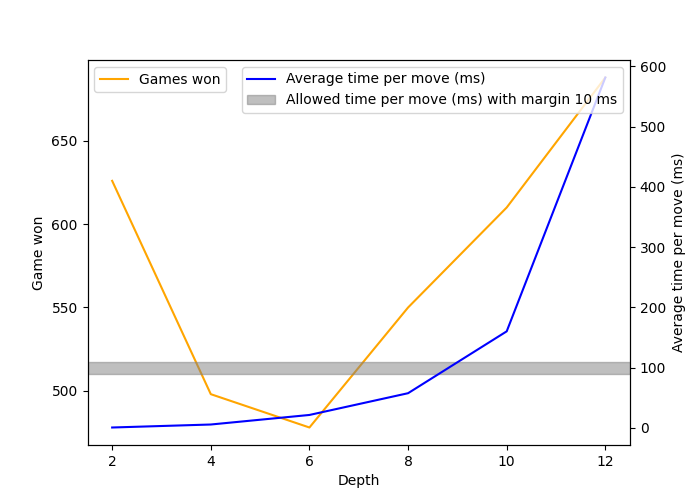
\includegraphics[width=0.8\textwidth]{../img/minimax_config_openworld.png}
  \caption{Comparison of win rates of different fixed depths parameters in minimax algorithm along with average time taken per ply}
  \label{minimaxOWDepth}
\end{figure}

Figure \ref{minimaxOWEval} illustrates the comparison between two heuristic evaluation functions, namely \texttt{basic} and \texttt{playout}, for the minimax algorithm with a fixed depth of 9. The left subplot shows the win rates for the two evaluation functions, and the right subplot displays the average time (ms) taken to make a move. It can be observed that the playout heuristic consistently outperforms the basic heuristic in terms of win rate, achieving almost twice the win rate of the basic heuristic. However, the playout heuristic is slower than the basic heuristic, as shown by the right subplot. Despite this, the playout heuristic still performs within the optimal time range of 100ms, making it the preferred choice for the tournament. As a result, the minimax agent will use the depth 9 and playout heuristic for the tournament.

\begin{figure}[h]
  \centering
  \captionsetup{justification=centering}
  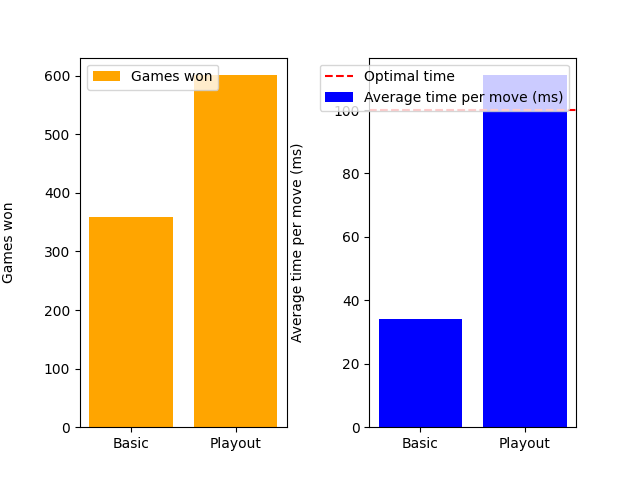
\includegraphics[width=0.8\textwidth]{../img/minimax_eval_openworld.png}
  \caption{Comparison of win rates and average time taken per ply of \texttt{basic} and \texttt{playout} evaluation functions in minimax algorithm}
  \label{minimaxOWEval}
\end{figure}


\subsection{Configuring MCTS Parameters}

In order to compare MCTS agents with other agents in the open world, it is necessary to determine the optimal values for the parameters \texttt{limit}, \texttt{c}, and \texttt{simulation}. To begin, the exploration constant was set to 1.41, which is typically the optimal value, and the simulation was set to greedy. With these parameters in place, an experiment was conducted using 1000 games to find the value of \texttt{limit} by trying various values of iterations to identify the optimal value. The results of this experiment are depicted in Figure \ref{mctsOWIterations}.

\begin{figure}[h]
  \centering
  \captionsetup{justification=centering}
  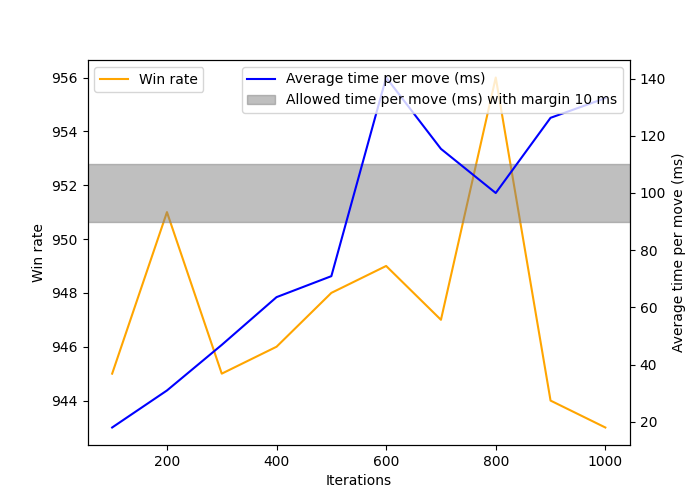
\includegraphics[width=0.8\textwidth]{../img/mcts_iterations_openworld.png}
  \caption{Comparison of win rates and average time taken per ply of different fixed iterations in MCTS algorithm}
  \label{mctsOWIterations}
\end{figure}

Similar to the minimax algorithm, it can be seen that an increase in the number of \texttt{iterations} generally results in a corresponding increase in the average time taken per move, as well as an increase in the win rate. By examining the shaded region in Figure \ref{mctsOWIterations}, which represents the optimal time per move, it can be determined that the optimal value for the \texttt{iterations} parameter is 800. This value results in the highest win rate and the lowest average time taken per move.

With the \texttt{iterations} parameter set to 800 and the \texttt{simulation} value remaining at greedy, a new experiment was conducted to determine the optimal value for the \texttt{c} exploration parameter in MCTS. The results of this experiment are shown in Figure 6. From the figure, it can be observed that the optimal value for the \texttt{c} parameter is 1.00, as it yields the highest win rate while still operating within the optimal average time per move.

\section{Closed world}
